\documentclass{oblivoir}
\usepackage{amsmath,amssymb,amsthm,kotex,paralist,kswrapfig}

\usepackage[skipabove=10pt,skipbelow=10pt,innertopmargin=10pt]{mdframed}

\usepackage{tabto,pifont}
\TabPositions{0.2\textwidth,0.4\textwidth,0.6\textwidth,0.8\textwidth}
\newcommand\tabb[5]{\par\bigskip\noindent
\ding{172}\:{\ensuremath{#1}}
\tab\ding{173}\:\:{\ensuremath{#2}}
\tab\ding{174}\:\:{\ensuremath{#3}}
\tab\ding{175}\:\:{\ensuremath{#4}}
\tab\ding{176}\:\:{\ensuremath{#5}}}

\newcommand\tabfive[5]{\par\medskip\noindent
\ding{172}\:\:{\ensuremath{#1}}\\
\ding{173}\:\:{\ensuremath{#2}}\\
\ding{174}\:\:{\ensuremath{#3}}\\
\ding{175}\:\:{\ensuremath{#4}}\\
\ding{176}\:\:{\ensuremath{#5}}}

\usepackage{enumitem}
\setlist[enumerate]{label=(\arabic*)}

\newcounter{num}
\newcommand{\defi}[1]
{\noindent\refstepcounter{num}\textbf{정의 \arabic{num}) #1}\par\noindent}
\newcommand{\theo}[1]
{\noindent\refstepcounter{num}\textbf{정리 \arabic{num}) #1}\par\noindent}
\newcommand{\exam}[1]
{\bigskip\bigskip\noindent\refstepcounter{num}\textbf{예시 \arabic{num}) #1}\par\noindent}
\newcommand{\prob}[1]
{\bigskip\bigskip\noindent\refstepcounter{num}\textbf{문제 \arabic{num}) #1}\par\noindent}
\newcommand{\proo}
{\bigskip\textsf{증명)}\par}

\newcommand{\procedure}[1]{\begin{mdframed}\vspace{#1\textwidth}\end{mdframed}}
\newcommand{\ans}{
{\par\raggedleft\textbf{답 : (\qquad\qquad\qquad\qquad\qquad\qquad)}\par}\bigskip\bigskip}
\newcommand\an[1]{\par\bigskip\noindent\textbf{문제 #1)}\\}

\newcommand{\pb}[1]%\Phantom + fBox
{\fbox{\phantom{\ensuremath{#1}}}}

\newcommand\ba{\,|\,}

\let\oldsection\section
\renewcommand\section{\clearpage\oldsection}

\let\emph\textsf
%%%%
\begin{document}

\title{규현 03 : 수학2 복습}
\author{}
\date{\today}
\maketitle
\tableofcontents
\newpage

%%
\section{집합}

\begin{mdframed}
%
\defi{집합과 원소}
어떤 조건이나 기준에 의하여 그 대상을 분명히 알 수 있는 것들의 모임을 \emph{집합}이라고 한다.
또 집합을 이루는 대상 하나하나를 그 집합의 \emph{원소}라고 한다.
\end{mdframed}

%
\prob{}
\begin{enumerate}
\item
\(10\)보다 작은 자연수의 모임	\tabto{0.6\textwidth}(집합이다, 집합이 아니다)
\item
\(1\)에 가까운 수의 모임		\tabto{0.6\textwidth}(집합이다, 집합이 아니다)
\item
성북구에 위치한 중학교의 모임	\tabto{0.6\textwidth}(집합이다, 집합이 아니다)
\item
수학 점수가 높은 학생의 모임	\tabto{0.6\textwidth}(집합이다, 집합이 아니다)
\end{enumerate}

\exam{}\label{set_notation_example}
%\(A\)를 `8의 약수들의 집합'이라고 할 때, 집합 \(A\)를 나타내는 방법에 대해 알아보자.
\(A\)를 `8의 약수들의 집합'이라고 하자.
\(A\)는 다음의 세 방법으로 나타낼 수 있다.
\begin{enumerate}
\item
\(A\)의 원소들을 일일이 나열하는 방법(원소나열법);
\[A=\{1,2,4,8\}\]
\item
\(A\)에 속하는 조건을 제시하는 방법(조건제시법);
\[A=\{x\;|\;x\text{는 8의 약수}\}\]
\item
그림으로 표현하는 방법(벤다이어그램);\\
\begin{center}
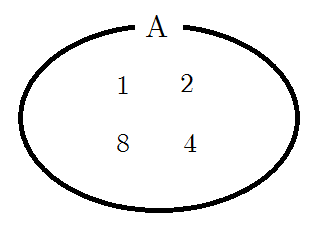
\includegraphics[width=0.3\textwidth]{venn}
\end{center}
\end{enumerate}

이때 \(2\)는 \(A\)의 원소이고, \(3\)은 \(A\)의 원소가 아니다.
이것을
\[2\in A,\qquad3\notin A\]
로 나타낸다.
또, \(B=\{x\ba x\text{는 }16\text{의 약수}\}\)라고 하면 \(B=\{1,2,4,8,16\}\)이다.
\(A\)의 모든 원소가 \(B\)에 속하는데 이것을
\[A\subset B\]
로 나타낸다.
이때 \(A\)는 \(B\)의 \emph{부분집합}이라고 한다.


%
\kswrapfig[Pos=r]{complement_example}{
\exam{}
전체집합 \(U=\{1,2,3,4,5,6\}\)의 두 부분집합 \(A=\{1,3,5\}\), \(B=\{2,3,4\}\)에 대하여 
\begin{align*}
A\cap B 	&=\phantom{\{3\}}\\
A\cup B 	&=\phantom{\{1,2,3,4,5\}}\\
A^c 		&=\phantom{\{2,4,6\}}\\
A-B 		&=\phantom{\{1,5\}}
\end{align*}
}

\begin{mdframed}
%
\theo{분배법칙, 드모르간의 법칙}\label{de_morgan}
세 집합 \(A\), \(B\), \(C\)에 대해
\begin{enumerate}
\item
\(A\cap(B\cup C)=(A\cap B)\cup(A\cap C)\)
\item
\(A\cup(B\cap C)=(A\cup B)\cap(A\cup C)\)
\item
\((A\cap B)^c=A^c\cup B^c\)
\item
\((A\cup B)^c=A^c\cap B^c\)
\end{enumerate}

\end{mdframed}
\begin{mdframed}
%
\theo{집합의 원소의 개수}
\[n(A\cup B)=n(A)+n(B)-n(A\cap B)\]
\end{mdframed}


%%
\section{명제}

\begin{mdframed}
%
\defi{명제}
그 내용이 참인지 거짓인지를 명확하게 판별할 수 있는 문장이나 식을 \emph{명제}라고 한다.
\end{mdframed}

\vspace{-10pt}
%
\prob{}
다음 중 명제인 것을 모두 찾고, 그것의 참, 거짓을 판별하여라.
\begin{enumerate}[itemsep=0pt]
\item
삼각형의 세 내각의 크기의 합은 \(180^\circ\)이다.
\item
\(x=2\)이면 \(2x+1=3\)이다.
\item
\(x-1\le3\)
\item
\(\frac1{100}\)은 \(0\)에 가까운 수이다.
\end{enumerate}

%
\exam{\(p\to q\)꼴의 명제}
명제
\begin{center}
\(x\)가 3의 약수이면 \(x\)는 6의 약수이다.
\end{center}
는 \(p\to q\) 꼴의 명제이다.
이때 \(p\)를 \emph{가정}, \(q\)를 \emph{결론}이라고 한다.
\(p\), \(q\)의 \emph{진리집합}을 각각 \(P\), \(Q\)라고 하면

%두 조건
%\begin{align*}
%p\::\:`x\text{는 3의 약수이다.'}\\
%q\::\:`x\text{는 6의 약수이다.'}
%\end{align*}
%에 대하여 \(p\to q\)는 참이다.
%이때, 이 명제의 가정 \(p\)와 결론 \(q\)의 진리집합을 각각 \(P\), \(Q\)라고 하면
\[P=\{1,3\},\quad Q=\{1,2,3,6\}\]
이다.
따라서 \(P\subset Q\)이므로 \(p\to q\)는 참이다.
\(p\to q\)가 참이면 \(p\Rightarrow q\)로 나타내고, \(p\)가 \(q\)이기 위한 \emph{충분조건}, \(q\)가 \(p\)이기 위한 \emph{필요조건}이라고 한다.

이 명제의 \emph{역}인
\begin{center}
\(x\)가 6의 약수이면 \(x\)는 3의 약수이다.
\end{center}
는 \(q\to p\)이고 이 명제는 거짓이다.
\(Q\not\subset P\)이기 때문이다.
따라서 \emph{원래 명제가 참이라고 해서 그 역도 참이라고 할 수는 없다.}

하지만 이 명제의 \emph{대우}인
\begin{center}
\(x\)가 6의 약수가 아니면 \(x\)는 3의 약수가 아니다.
\end{center}
는 참이다.
일반적으로 \emph{원래 명제가 참이면 그 대우는 무조건 참이다.}

%또한 \(q\to p\)는 거짓이다.
%원소 \(2\)는 6의 배수이기는 하지만 \(3\)의 배수라고는 할 수 없기 때문이다.
%이때 \(Q\not\subset P\)이다.



\begin{mdframed}
%
\defi{절대부등식}
부등식 \((x-1)^2\ge0\), \(x^2+1>0\), \(|x-1|+1>0\)은 모두 \(x\)에 어떤 실수를 대입해도 항상 성립한다.
이와 같이 문자에 어떤 실수를 대입해도 항상 성립하는 부등식을 \emph{절대부등식}이라고 한다.
\end{mdframed}

\begin{mdframed}
%
\theo{산술-기하 부등식}
\(a>0\), \(b>0\)이면
\[a+b\ge2\sqrt{ab}.\]
(단 등호는 \(a=b\)일 때 성립한다.)
\end{mdframed}


\begin{mdframed}
%
\theo{코시-슈바르츠 부등식}
실수 \(a\), \(b\), \(x\), \(y\)에 대하여
\[(a^2+b^2)(x^2+y^2)\ge(ax+by)^2\]
(단 등호는 \(a:b=x:y\)일 때 성립한다.)
\end{mdframed}

%
\exam{}
\(x^2+y^2=4\)일 때, 다음을 구하여라.
\begin{enumerate}
\item
\(xy\)의 최댓값
\item
\(3x+4y\)의 최댓값
\end{enumerate}
\begin{mdframed}
\begin{enumerate}
\item
\(4=x^2+y^2\ge2\sqrt{x^2\times y^2}=2|xy|\)
에서 \(|xy|\le2\).\\
따라서 \(-2\le xy\le2\). \(xy\)의 최댓값은 \(2\)이다.
\item
\((3^2+4^2)(x^2+y^2)\ge(3x+4y)^2\)에서 \((3x+4y)^2\le100\).\\
\(-10\le3x+4y\le10\). 따라서 \(3x+4y\)의 최댓값은 \(10\)이다.
\end{enumerate}
\end{mdframed}

%%
\section{함수}
%
\exam{}
오른쪽 그림과 같은 함수 \(f:X\to Y\)에서 \emph{정의역}은 \(X=\{1,2,3\}\)이고 \emph{공역}은 \(Y=\{a,b,c\}\)이다.
또

\kswrapfig[Pos=r]{discreet}{
\begin{align*}
f(1)&=c\\
f(2)&=b\\
f(3)&=a
\end{align*}
이므로 함숫값들의 집합인 \emph{치역}은 \(\{a,b,c\}\)로 공역과 같다.
또
\[x_1\neq x_2\Rightarrow f(x_1)\neq f(x_2)\]
이므로 \emph{일대일 함수}이고, 또한 \emph{일대일 대응}이기도 하다.
}

%
\exam{}
정의역과 공역이 모두 실수 집합인 함수 \(g(x)=x^2\)의 \emph{그래프}는 오른쪽 그림과 같다.

\kswrapfig[Pos=r]{continuous}{
이 함수의 치역은 \(\{y\ba y\ge0\}\)이므로 공역과 같지 않다.
또, 정의역의 서로 다른 두 원소 \(-2\)과 \(2\)에 대해 \[g(-2)=g(2)\]이므로 이 함수는 일대일 함수가 아니다.

이 함수는 \(x\le0\)일 때, \emph{감소함수}이고, \(x\ge0\)일 때, \emph{증가함수}이다.
또, \(y\)축을 기준으로 대칭이므로 \emph{우함수}이다.
}

%
\exam{합성함수}
\kswrapfig[Pos=r]{composition}{
오른쪽 그림과 같이 두 함수 \(f:X\to Y\), \(g:Y\to Z\)를 합성하면 새로운 함수
\[g\circ f:X\to Z\]
를 얻는다.
이 함수는
\[
(g\circ f)(x)=g(f(x))
\]
로 정의된 함수로
\begin{align*}
(g\circ f)(1)&=g(f(1))=g(a)=2\\
(g\circ f)(2)&=g(f(2))=g(d)=5\\
(g\circ f)(3)&=g(f(3))=g(b)=7
\end{align*}
이다.
}

\end{document}